%pour les annexes, évidemment


\begin{figure}[h!]
\centering
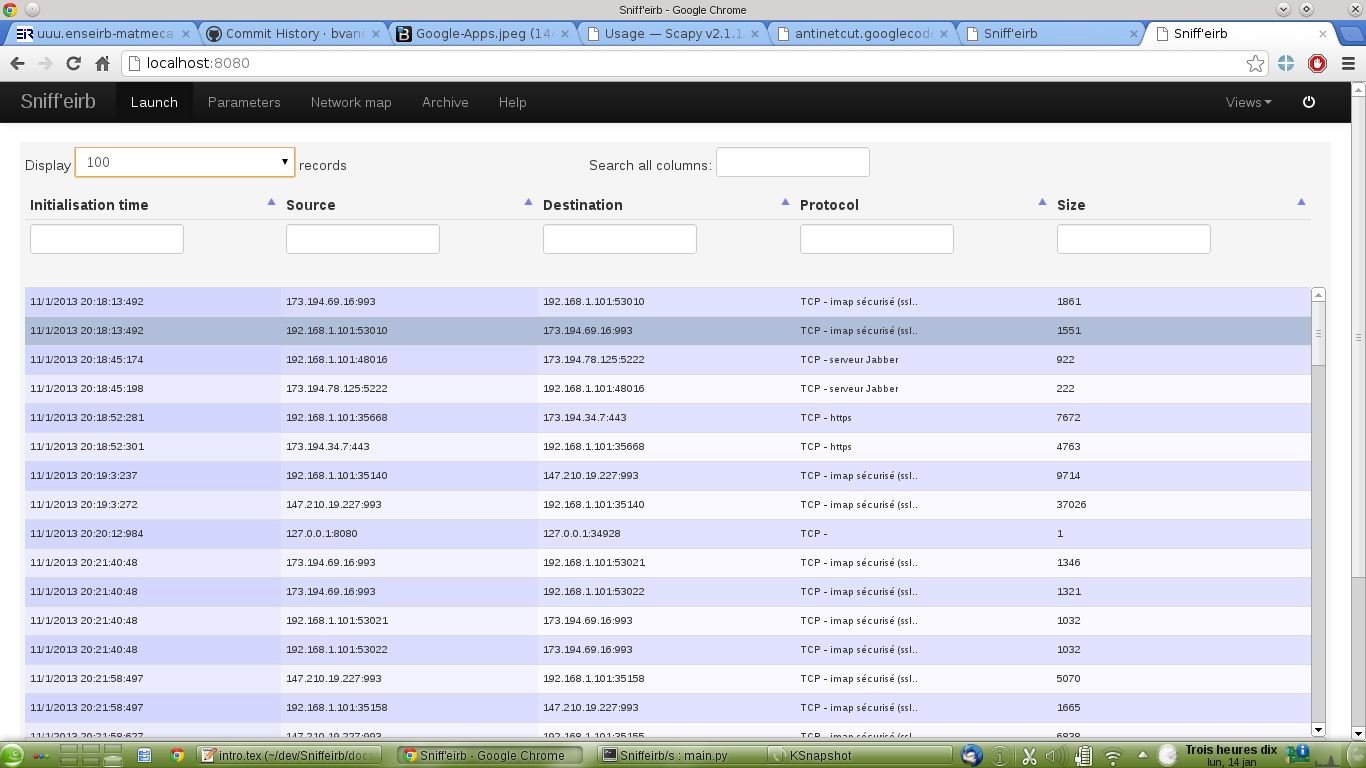
\includegraphics[scale=0.5]{NormalView.png}
\caption{Page d'accueil}
\label{NormalView}
\end{figure}

\begin{figure}[h!]
\centering
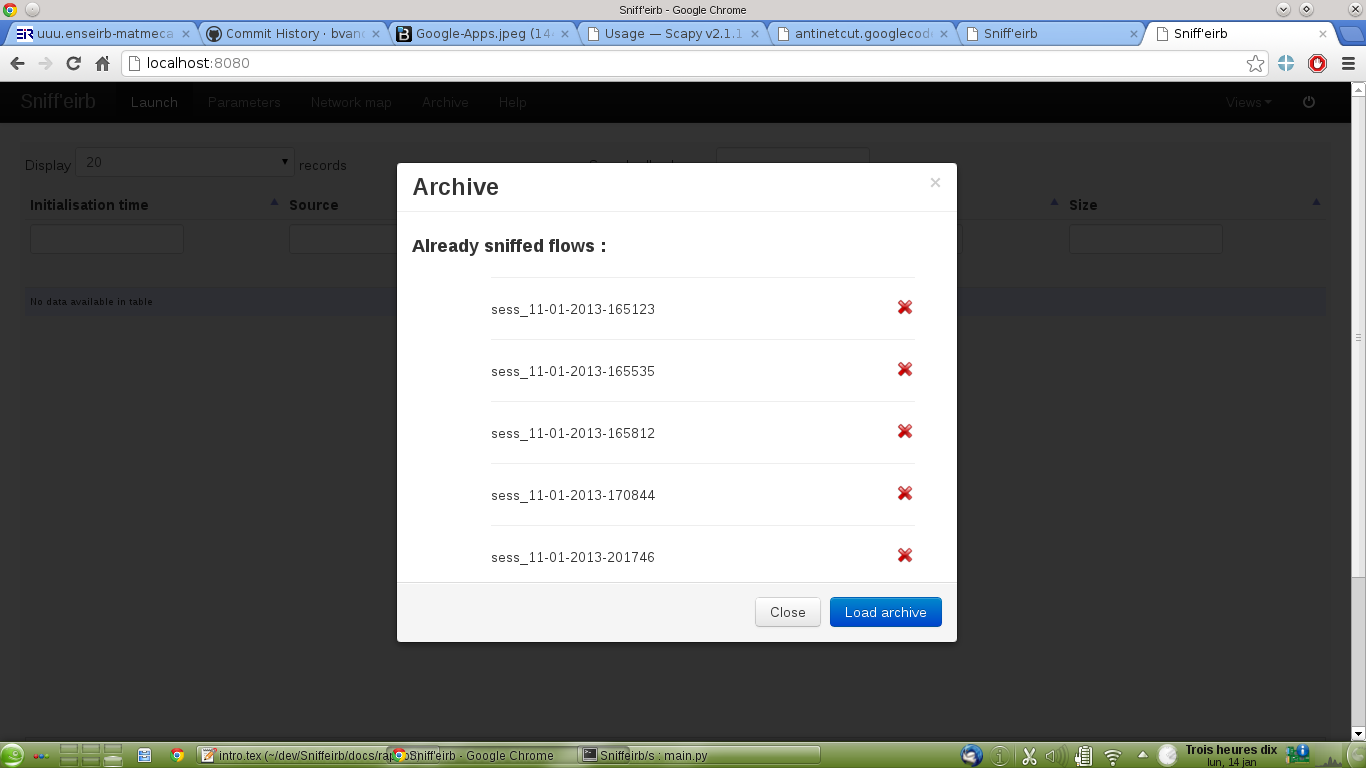
\includegraphics[scale=0.5]{Archive.png}
\caption{Archive}
\label{Archive}
\end{figure}

\begin{figure}[h!]
\centering
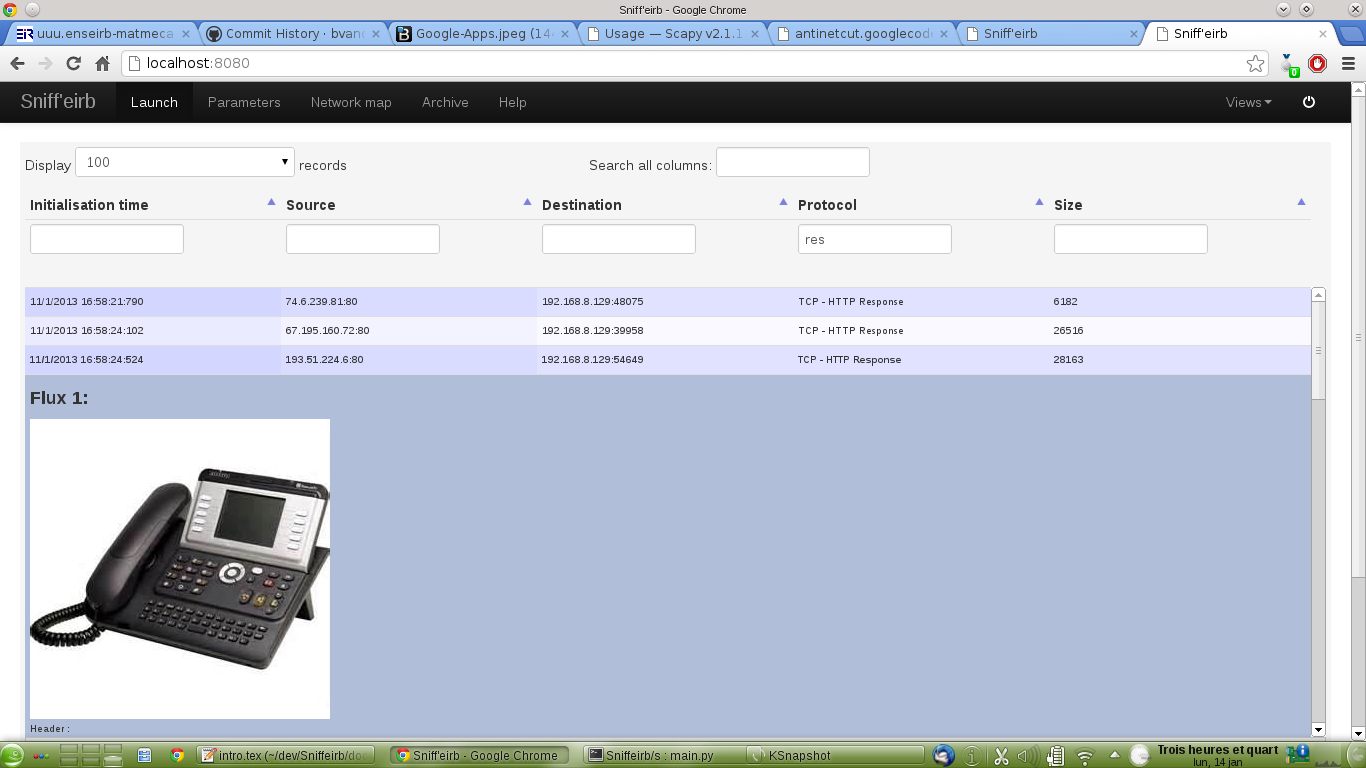
\includegraphics[scale=0.5]{DetailView.png}
\caption{Vu d'une image reconstruite}
\label{DetailView}
\end{figure}


\begin{figure}[h!]
\centering
\begin{verbatim}
{
        "_id" : ObjectId("50edc0fe10b95715ceddf583"),
        "dport" : 80,
        "dst" : "50.57.168.107",
        "initTS" : 1357758718.609804,
        "packets" : [
                {
                        "ack" : 0,
                        "flags" : "S",
                        "ts" : 1357758718.609804,
                        "seq" : NumberLong("3047389275")
                },
                {
                        "ack" : NumberLong("3368619615"),
                        "flags" : "A",
                        "ts" : 1357758718.736191,
                        "seq" : NumberLong("3047389276")
                },
                {
                        "ack" : NumberLong("3368619615"),
                        "flags" : "A",
                        "ts" : 1357758722.540476,
                        "seq" : NumberLong("3047389276")
                }
        ],
        "proto" : "TCP",
        "session" : "sess_09-01-2013-201054",
        "sport" : 53879,
        "src" : "192.168.1.101",
        "type" : "IP"
}

\end{verbatim}
\caption{Extrait de la base Mongo : un document}
\end{figure}

